\section{Spazi metrici e normati}
\subsection{Norme e metriche}

\begin{definition}
	
	$X$ spazio vettoriale su $\mathbb{R}$ o $\mathbb{C}$. Una norma su $X$ è una funzione $\parallel \cdot \parallel : X \rightarrow \mathbb{R}$ tale che 
	\begin{enumerate}
		\item $\parallel x \parallel \geq 0 \quad \forall \ x \in X$ e $\parallel x \parallel = 0 \iff x = 0$
		
		\item $\parallel \lambda x \parallel = |\lambda| \parallel x \parallel \quad \forall$ scalare $\lambda$ e $\forall \ x \in X$
		
		\item $\parallel x+y \parallel \leq \parallel x \parallel + \parallel y \parallel \quad \forall x,y \in X$ (disuguaglianza triangolare)
	\end{enumerate}
	La coppia ($X,\parallel \cdot \parallel$) si dice spazio normato
\end{definition}


\begin{exbar}
\begin{itemize}
	\item $(\mathbb{R}, |\cdot|)$ è spazio normato
	
	\item $(\mathbb{R}^n, |\cdot|)$ è spazio normato (norma euclidea)
	\begin{gather*}
		\overline{x} = (x_1,...,x_n) \in \mathbb{R}^n
		\\ \big| \overline{x} \big| = \sqrt{\sum_{i=1}^{n }x_i^2}= \sqrt{ \langle \overline{x}, \overline{x} \rangle}
	\end{gather*} 
	
	dove, se $\overline{x} = (x_1,...,x_n)$ e $\overline{y} = (y_1,...,y_n)$
	\begin{gather*}
	\langle  \overline{x}, \overline{y} \rangle = \sum_{i=1}^{n} x_i y_i 
	\\
	\text{prodotto scalare tra } \overline{x} \text{ e } \overline{y}
	\end{gather*}

	\item $(\mathbb{R}^n, \parallel \cdot \parallel_{\infty})$ è spazio normato
	\begin{gather*}
		\overline{x} = (x_1,...,x_n) 
		\\
		\parallel \overline{x} \parallel_\infty = \max_{i=1,...,n} |x_i|
	\end{gather*}
	
	(Per casa dimostrare che è una norma)
	
	\item $(\mathbb{R}^n,\parallel\cdot\parallel_1)$ è spazio normato
	\begin{gather*}
		\overline{x} = (x_1,...,x_n)
		\\
		\parallel \overline{x} \parallel_1 \sum_{i=1}^{n} |x_i| = |x_1| + |x_2| + \ldots + |x_n|
	\end{gather*}
	
	
	Se $n=2$ e $(x,y)\in \mathbb{R}^2$
	\begin{gather*}
		\parallel (x,y) \parallel_\infty = \max \{ |x|,|y| \}
		\\
		\parallel (x,y) \parallel_1 = |x| + |y|
	\end{gather*}
	
	\begin{center}
		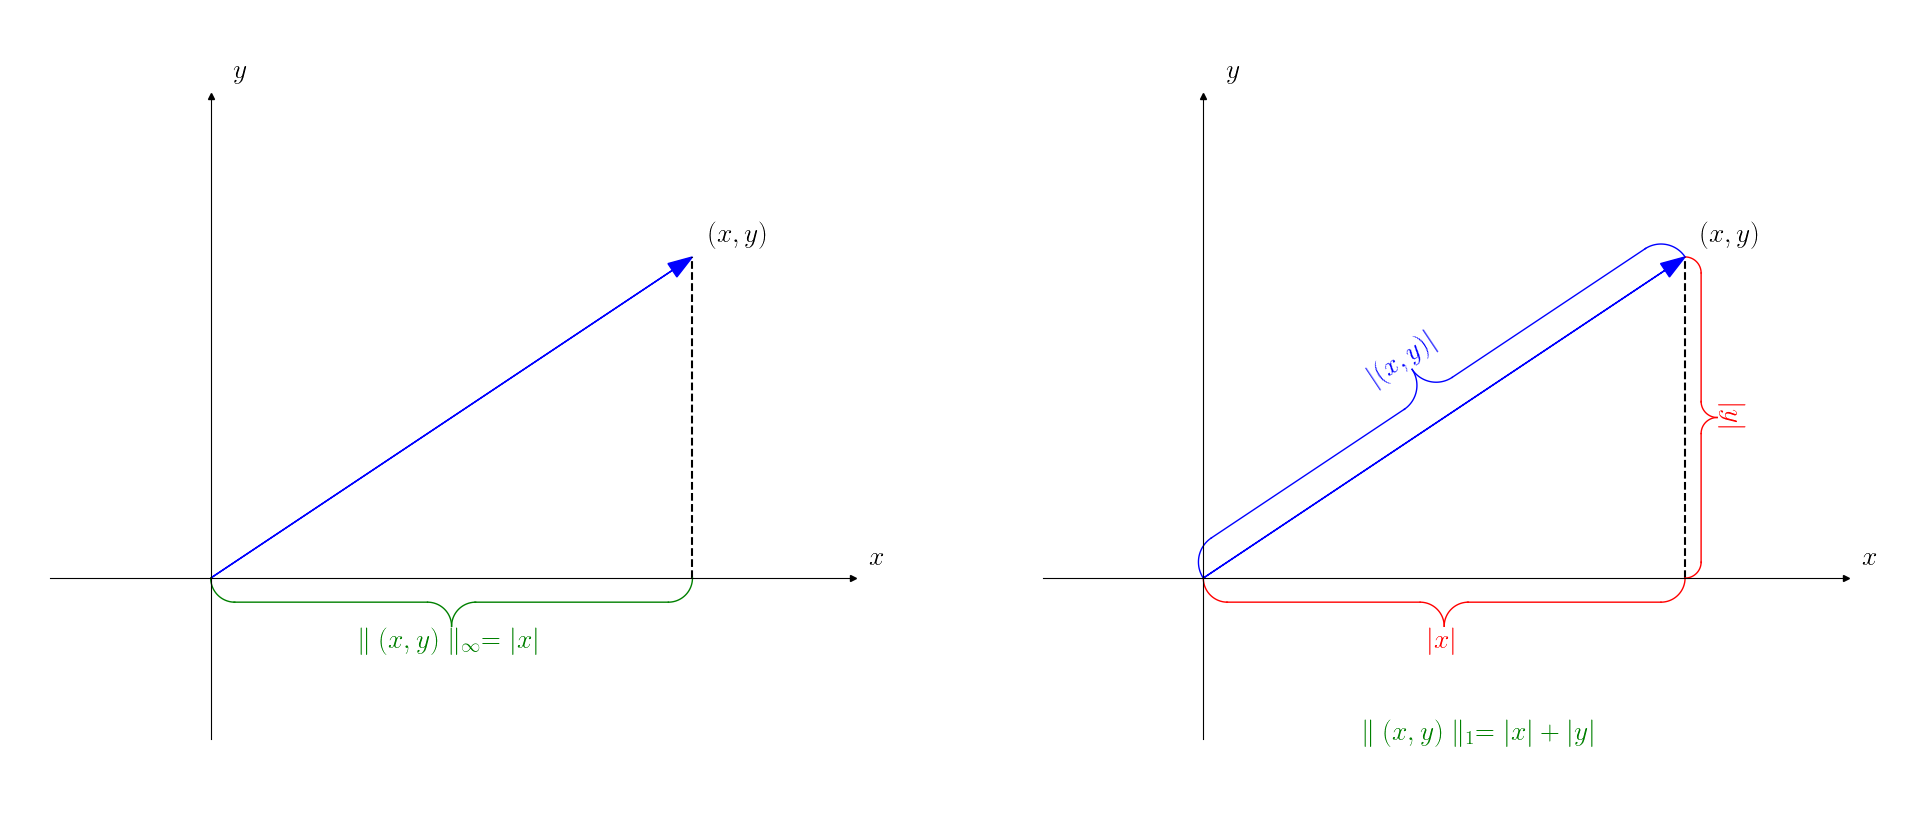
\includegraphics[width=\linewidth]{spazi_metrici_e_normati/pag126}
		\label{fig:pag126}
	\end{center}
	\begin{gather*}
		\parallel \overline{x} \parallel_p = \left( \sum_{i=1}^{n} |x_i|^p \right)^{\frac{1}{p}} \quad p \geq 1
		\\
		\parallel \overline{x} \parallel_\infty = \lim_{p \rightarrow +\infty} \parallel \overline{x} \parallel_p
	\end{gather*}
	$(\mathbb{R}^n, \parallel \cdot \parallel_p)$ è spazio normato

	\item $C^0 \left( [0,1] \right)$
	\begin{align*}
		&\parallel f \parallel_\infty = \sup_{x \in [0,1]} |f(x)| (=\max_{x \in [0,1]} |f(x)|)
		\\
		&\parallel f \parallel_1 = \int_{0}^{1} |f(x)| \ \mathrm{d}x
		\\
		&\parallel f \parallel_p = \left( \int_{0}^{1} |f(x)|^p \ \mathrm{d}x \right)^{\frac{1}{p}} \qquad p \geq 1
	\end{align*}

sono tute norme su $C^0 ([0,1])$
\end{itemize}
\end{exbar}


\begin{exbar}
\begin{example}
	Facciamo vedere che $\parallel \cdot \parallel_\infty$ su $C^0 ([0,1])$ è una norma
	\begin{enumerate}
		\item $\parallel f \parallel_\infty \geq 0 \qquad$ (banale)
		
		$\parallel f \parallel_\infty =  0 \iff f(x) = 0 \qquad \forall \ x \in [0, 1]$
		
		$\parallel f \parallel_\infty =  0 \iff \sup_{x \in [0,1]} |f(x)| = 0$
		
		$\iff 0 \leq |f(x)| \leq 0 \quad \forall \ x \in [0,1] \iff f(x) = 0 \qquad \forall \ x \in [0,1]$
		
		\item $\parallel \lambda f \parallel_\infty = |\lambda| \parallel f \parallel_\infty \qquad \forall \lambda \in \mathbb{R}$ e $\forall f \in C^0 ([0,1])$
		
		$\parallel \lambda f \parallel_\infty = \sup_{x \in[0,1]} |\lambda f(x)| = \sup_{x\in[0,1]} |\lambda| \ |f(x)| = |\lambda| \sup_{x\in[0,1]} |f(x)| = |\lambda| \parallel f \parallel_\infty$
		
		\item $\parallel f+g \parallel_\infty \leq \parallel f \parallel_\infty + \parallel g \parallel_\infty \qquad \forall f,g \in C^0 ([0,1])$
		
		$\parallel f+g \parallel_\infty = \sup_{x\in[0,1]} |f(x) + g(x)|$
		
		$|f(x) + g(x)| \distr |f(x)| + |g(x)| \leq \sup_{y\in[0,1]} |f(y)| + \sup_{y\in[0,1]} |g(y)| =  \parallel f \parallel_\infty + \parallel g \parallel_\infty \qquad \forall \ x \in [0,1]$
		
		$\parallel f+g \parallel_\infty = \sup_{x\in[0,1]} |f(x) + g(x)| \leq \parallel f \parallel_\infty + \parallel g \parallel_\infty$\\
	\end{enumerate}
\end{example}
\end{exbar}
	

\begin{exbar}
\begin{example}
		Facciamo vedere che $\parallel f\parallel_1 = \int_{0}^{1} |f(x)| \ \mathrm{d}x$
		
		è una norma
	\begin{enumerate}
		\item $\parallel f \parallel_1 \geq 0 \qquad \forall f \in C^0 ([0,1]) \text{ banale}$
		
		Dimostriamo che $\parallel f \parallel_1 = 0 \iff f(x) = 0 \qquad \forall \ x \in [0,1]$
		
		$\Leftarrow) f(x) = 0 \qquad \forall \ x \in[0,1]$
		
		$\parallel f \parallel_1 = \int_{0}^{1} 0 \ \mathrm{d}x = 0$
		
		$\Rightarrow)$ Sia $\parallel f \parallel_1 = 0$ e dimostriamo che $f(x) = 0 \qquad \forall \ x \in [0,1]$
		
		$\int_{0}^{1} |f(x)| \ \mathrm{d}x = 0$
		
		Se $\exists \ x_0 \in [0,1]$ tale che $|f(x_0)| \neq 0$ allora $\exists$ un intorno $U$ di $x_0 $ tale che $|f(x)| \geq \frac{|f(x_0)|}{2}$ $\qquad \forall x \in U \cap [0,1]$ 
		
		\begin{itemize}
			\item $U = \ ]x_0 - \delta, x_0 + \delta[ \ \subseteq [0,1]$
	
			\item $x_0=0$
			
			$U= \ ]0 - \delta, 0 + \delta[$
			
			$U \cap [0,1] = [0, \delta[$
			
			\item $x_1 = 1$
			 $U= \ ]1 - \delta, 1 + \delta[$
			 
			$U \cap [0, 1] = \ ]1 - \delta, 1]$
		\end{itemize}
		
		cioè in ogni caso $U \cap [0,1]$ è un intervallo di ampiezza almeno $\frac{\delta}{2}>0$
		
		\begin{equation*}
			\parallel f\parallel_1 = \int_{0}^{1} |f(x)| \ \mathrm{d}x \geq \int_{U \cap [0,1]} |f(x)| \ \mathrm{d}x \geq \int_{U \cap [0,1]} \frac{|f(x_0)|}{2} \ \mathrm{d}x \geq \frac{\delta}{4} |f(x_0)| > 0
		\end{equation*}
		
		il che è assurdo, perché $\parallel f\parallel_1 = 0$
		
		\item $\parallel \lambda f \parallel_1 = \int_{0}^{1} |\lambda f(x)| \ \mathrm{d}x = |\lambda| \int_{0}^{1} |f(x)| \ \mathrm{d}x = |\lambda| \parallel f \parallel_1 \qquad \lambda \in \mathbb{R}$
		
		\item $f,g \in C^0 ([0,1])$
		
		$\parallel f+g \parallel_1 = \int_{0}^{1} |f(x) + g(x)| \ \mathrm{d}x \leq \int_{0}^{1} (|f(x)| + |g(x)|) \ \mathrm{d}x = \parallel f \parallel_1 + \parallel g \parallel_1$
		
		$\Rightarrow$ vale la disuguaglianza triangolare
	\end{enumerate}
\end{example}
\end{exbar}


\begin{attbar}
	Dato uno spazio normato $(X, \parallel \cdot \parallel)$ posso definire la distanza tra due vettori $x,y \in X$ come $d(x,y)= \parallel x-y \parallel$, lunghezza del vettore $x-y$
	\begin{center}
		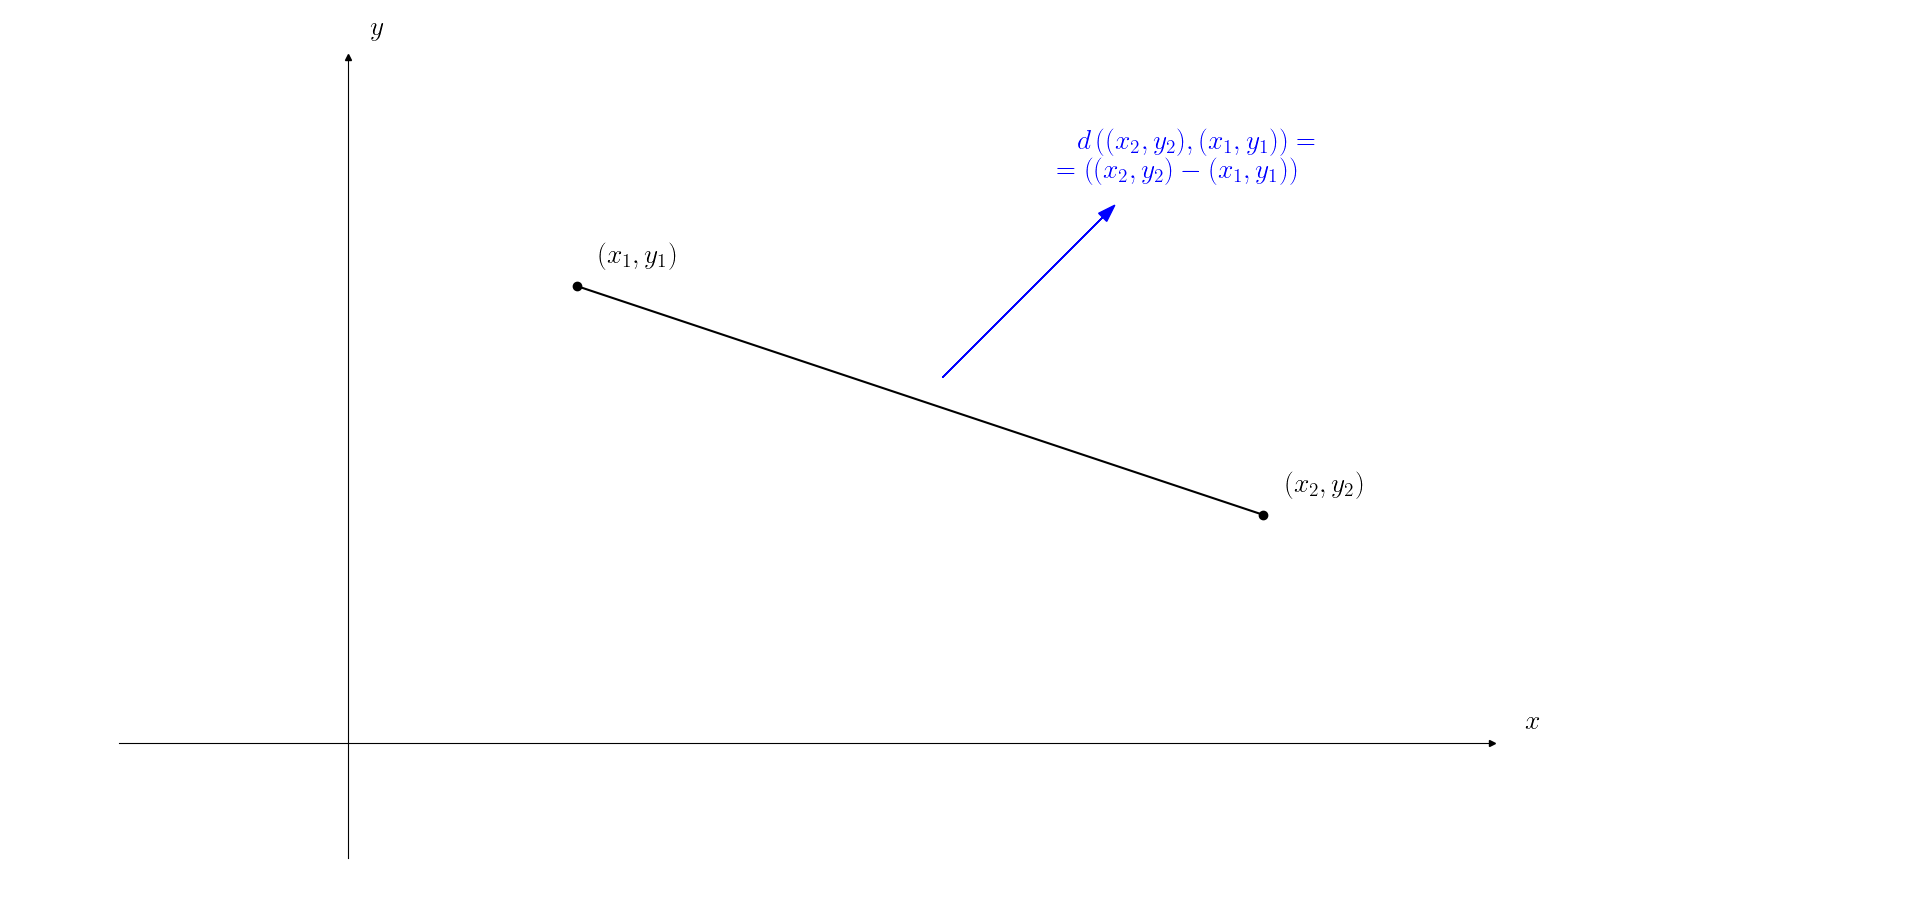
\includegraphics[width=0.75\linewidth]{spazi_metrici_e_normati/pag131}
		\label{fig:pag131}
	\end{center}
\end{attbar}


\begin{definition}
	$X$ insieme non vuoto. Una distanza o metrica su $X$ è una funzione $d:X \times X \rightarrow \mathbb{R}$ tale che
	\begin{enumerate}
		\item $d(x,y) \geq 0 \qquad \forall \ x,y \in X $ e $d(x,y) = 0 \iff x = y$
		\item $d(x,y) = d(y,x)$ (proprietà simmetrica)
		\item Disuguaglianza triangolare $d(x,y) \leq d(x,z) + d(z,y) \qquad \forall \ x,y,z \in X$
	\end{enumerate}
	
	La coppia $(X,d)$ si dice \textbf{spazio metrico}.
\end{definition}



$(X, \parallel \cdot \parallel)$ normato

$d(x,y)=\parallel x-y \parallel$ è metrica, allora
\begin{enumerate}
	\item $d(x,y)\geq 0$ banalmente 
	$d(x,y) = \parallel x-y \parallel = 0 \iff x-y = 0 \iff x = y$
	\item $d(x,y) = \parallel x-y \parallel = \parallel y-x \parallel = d(y,x)$
	\item $d(x,y) = \parallel x-y \parallel = \parallel (x-z) + (z-y) \parallel \leq \parallel x-z \parallel + \parallel z-y \parallel = d(x,z) + d(y,z)$
\end{enumerate}

Dato uno spazio vettoriale $X$ e $d$ metrica su $X$, esiste una norma $\parallel \cdot \parallel$ su $X$ tale che $d(x,y) = \parallel x-y \parallel$?

No, esistono metriche dentro lo spazio vettoriale che non derivano da una norma.


\begin{exbar}
\begin{example}
	$\mathbb{R}, \quad 0 < p < 1 , \quad d(x,y) = |x-y|^p$. 
	
	Allora $d$ è una metrica, che non deriva da una norma.
	
	Se esistesse una norma $\parallel \cdot \parallel$ su $\mathbb{R}$ tale che $d(x,y) = \parallel x-y \parallel$, allora, fissato $\lambda \in \mathbb{R}$,
	\begin{gather*}
		d(\lambda x, \lambda y) = \parallel \underbrace{\lambda x - \lambda y}_{\lambda (x - y)} \parallel \uppercomment{=} {\text{seconda}} {\text{proprietà di }\parallel \cdot \parallel} |\lambda| \parallel x-y \parallel = |\lambda | \ d(x,y)
		\\
		d(\lambda x, \lambda y) = |\lambda x - \lambda y|^p = |\lambda|^p |x-y|^p = |\lambda|^p d(x,y) \neq |\lambda| \ d(x,y) \text{ se } |\lambda \neq 1,0|
	\end{gather*}
	
	Facciamo vedere che $d(x,y) = |x-y|^p$ è una distanza, $0 < p < 1$
	\begin{enumerate}
		\item $d(x,y) \geq 0$ banale
		
		$d(x,y) = 0 \iff |x-y|^p = 0 \iff |x-y| = 0 \iff x = y$
		
		\item $d(x,y) = d(y,x)$ banale
		
		\item Disuguaglianza triangolare
		
		Dobbiamo dimostrare che $\forall \ x,y,z \in \mathbb{R}$ vale
		\begin{gather*}
			d(x,y) \leq d(x,z) + d(z,y)
			\\
			|x-y|^p \leq |x-z|^p + |z-y|^p
			\\
			|x-y|^p \distr (|x-z| + |y-z|)^p
		\end{gather*} 
	
		Se dimostro che $( \underbrace{|x-z|}_{= a} + \underbrace{|y-z|}_{=b})^p \leq |x-z|^p + |z-y|^p$, sono a posto $\forall \ x,y,z \in \mathbb{R}$ con $0<p<1$.
		
		Devo dunque dimostrare che $(a+b)^p \leq a^p + b^p \qquad \forall \ a,b \in \mathbb{R}^{\geq 0}$.
		
		Se $a=0$ o $b=0$, banale
		
		Siano $a,b \neq 0$
		\begin{gather*}
		(a + b)^p \leq a^p + b^p \qquad /.\frac{1}{b^p}
		\\
		\iff \frac{(a+b)^p}{b^p} \leq \frac{a^p}{b^p} + 1 \iff \left( \frac{a+b}{b} \right)^p \leq \left( \frac{a}{b} \right)^p + 1 \iff \left( \frac{a}{b} + 1 \right)^p \leq \left( \frac{a}{b} \right)^p + 1 \qquad \forall \ a,b > 0
		\end{gather*}
		
		Posto $\lambda = \frac{a}{b}>0$
		\begin{gather*}
		\left( \frac{a}{b} + 1 \right)^p \leq \left( \frac{a}{b} \right)^p + 1 \qquad \forall \ a,b>0 \iff (\lambda + 1)^p \leq \lambda^p + 1 \qquad \forall \ \lambda > 0
		\\
		(\lambda + 1)^p - \lambda^p \leq 1
		\\
		f(\lambda) = (\lambda + 1)^p -\lambda^p \qquad f:\mathbb{R}^{\geq 0} \rightarrow \mathbb{R}
		\\
		f(\lambda) \leq 1 = f(0)
		\\
		f'(\lambda) 
		\lowercomment{=} {\myarrow[270]} {\lambda \neq 0} p \ (\lambda + 1)^{p - 1} - p \ \lambda^{p - 1} 
		= p \ [(\lambda + 1)^{p - 1} - \lambda^{p - 1}] 
		= p \ \lambda^{p - 1} \left[ \left( \frac{\lambda + 1}{\lambda} \right)^{p-1} - 1 \right] 
		\\
		=  p \ \lambda^{p - 1} \left[ \underbrace{ \left(  1 + \frac{1}{\lambda} \right) ^{\overbrace{p - 1}^{<0}} }_{<1} - 1 \right] < 0 \qquad \forall \ \lambda > 0
 		\end{gather*}
		
		$f$ è decrescente e quindi $\forall \ \lambda > 0 \Rightarrow f(\lambda) \leq f(0)$, come si voleva.
	\end{enumerate}
\end{example}
\end{exbar}


\subsection{Topologia}

$(x,d)$ spazio metrico.

\begin{definition}
	
\end{definition}
	Sia $x \in X, r >0$, allora $B_r(x) = \{ y \in X | d(x,y) < r \}$ si dice \textbf{palla (aperta)} di centro $x$ e raggio $r$.

	
\begin{exbar}
	\begin{gather*}
		(\mathbb{R}^2, | \cdot |), \qquad \mathbb{R}^2 \text{ con norma euclidea}
		\\
		B_r (0,0), \qquad r > 0
		\\
		B_r (0,0) 
		= \{ (x,y) \in \mathbb{R}^2 \big| d((x,y), (0,0)) < r \} 
		= \{ (x,y) \in \mathbb{R}^2 \big| |(x,y)-(0,0)| < r \} =
		\\ 
		= \{ (x,y) \in \mathbb{R}^2 \big| \sqrt{x^2+y^2} < r\}
	\end{gather*}
	\begin{center}
		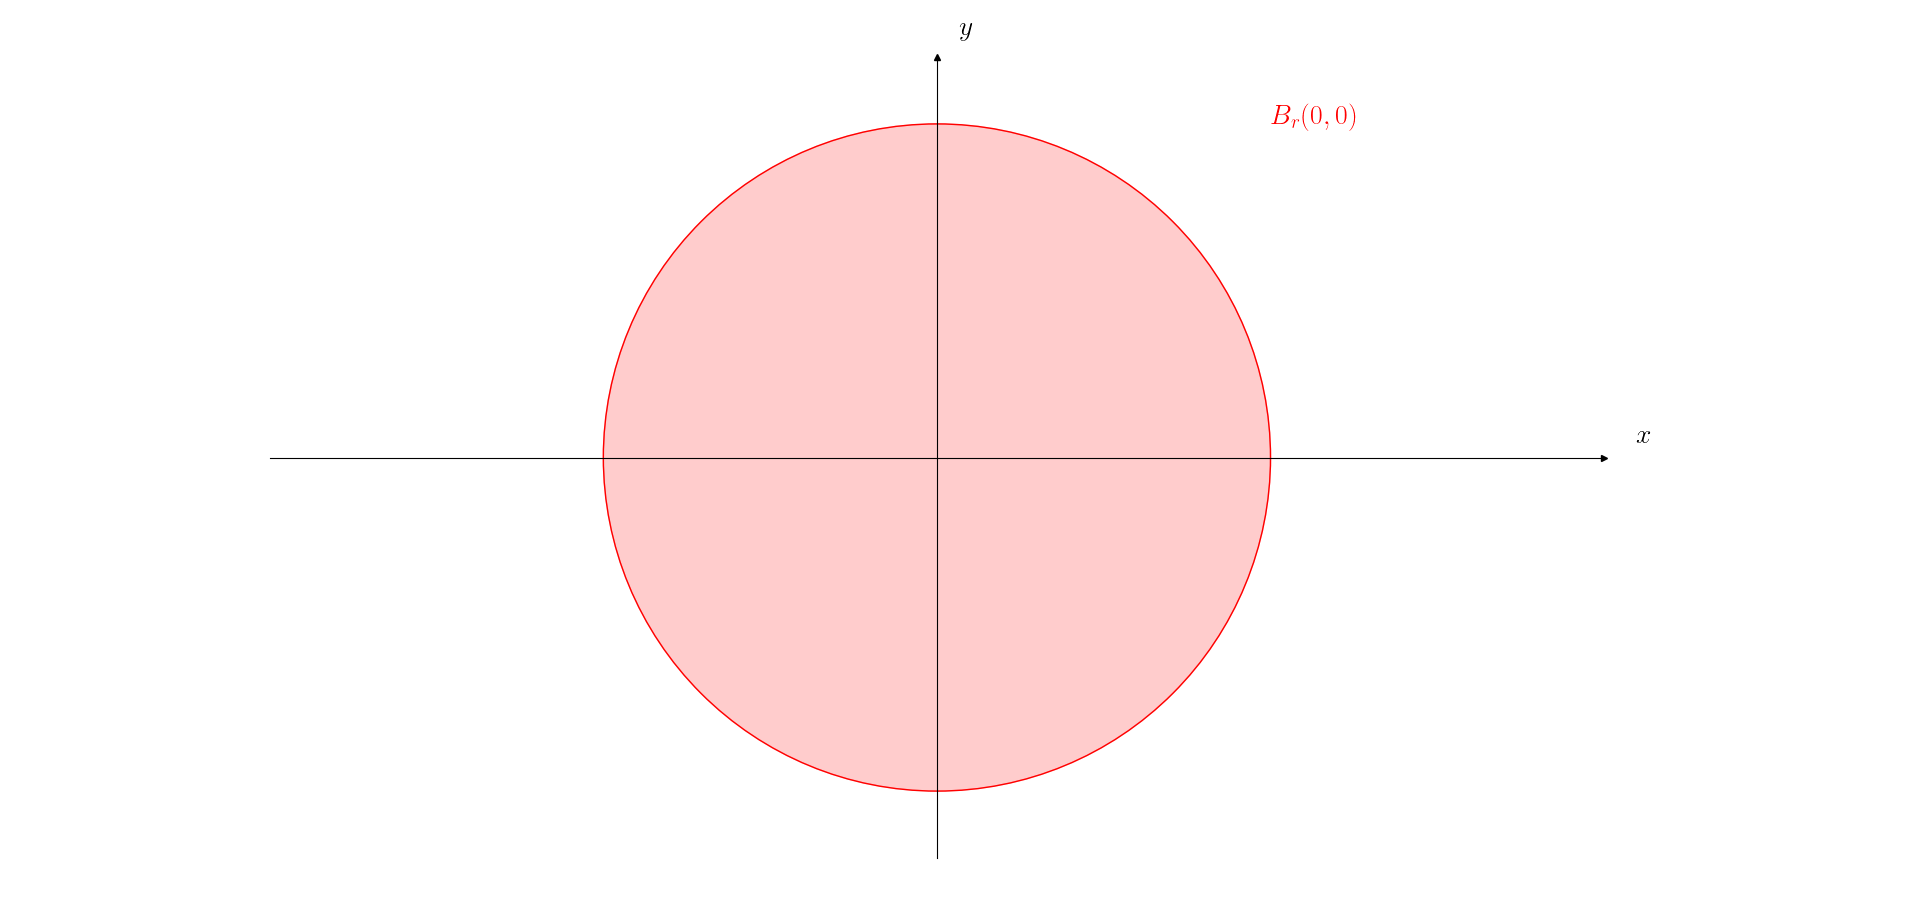
\includegraphics[width=0.75\linewidth]{spazi_metrici_e_normati/pag137circle}
		\label{fig:pag137circle}
	\end{center}
	
	\begin{gather*}
	 	(\mathbb{R}^2, \parallel \cdot \parallel_\infty)
	 	\\
		\parallel (x,y) \parallel_\infty = \max \{|x|,|y|\} 
		\\
		B_r^\infty (0,0) 
		= \{ (x,y) \in \mathbb{R}^2 \big| \parallel(x,y) - (0,0) \parallel_\infty < r \} 
		= \{ (x,y) \in \mathbb{R}^2 \big| \max \{|x|,|y| \} < r \} =
		\\
		= \{ (x,y) \in \mathbb{R}^2 \big| |x|,|y| < r\}
	\end{gather*}
	\begin{center}
		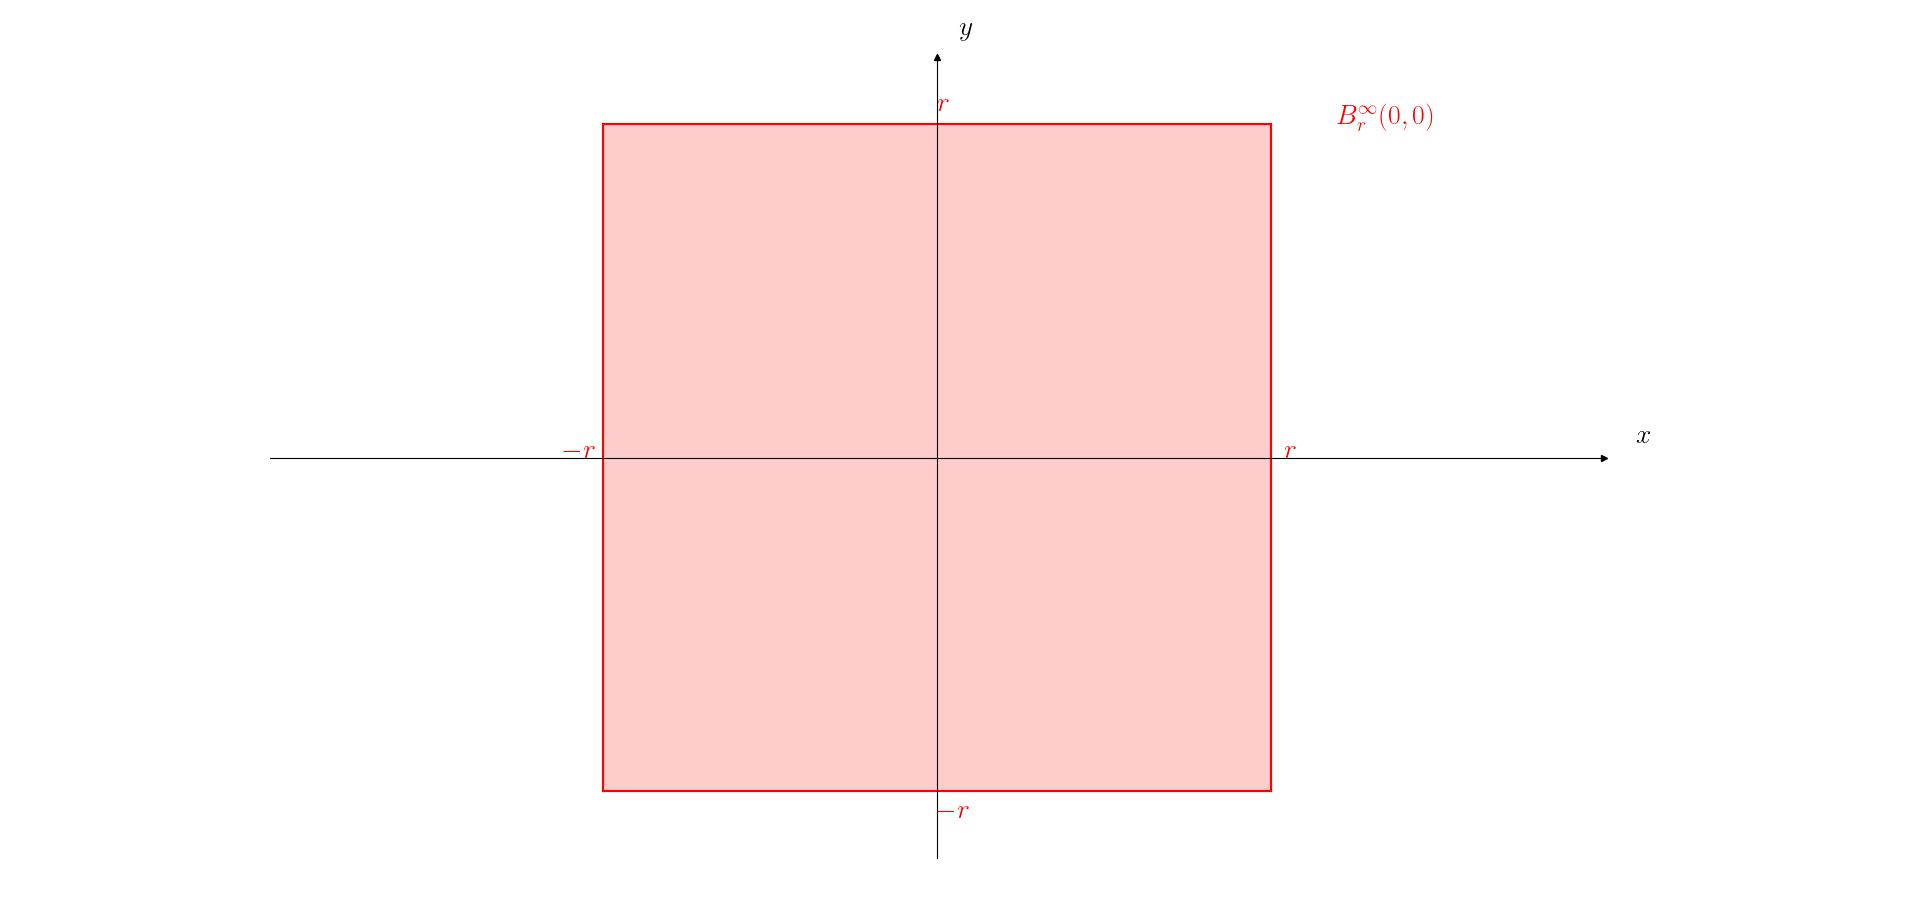
\includegraphics[width=0.75\linewidth]{spazi_metrici_e_normati/pag137square}
		\label{fig:pag137square}
	\end{center}
	
	\begin{gather*}
		(\mathbb{R}^2, \parallel \cdot \parallel_1)
		\qquad
		\parallel (x,y) \parallel_1 = |x| + |y| 
		\\
		B_r^1 (0,0) = \{(x,y) \in \mathbb{R}^2 \big| \parallel (x,y) - (0,0) \parallel_1 < r \} 
		= \{(x,y) \in \mathbb{R}^2 \big| |x| + |y| < r \}
	\end{gather*}
	\begin{center}
		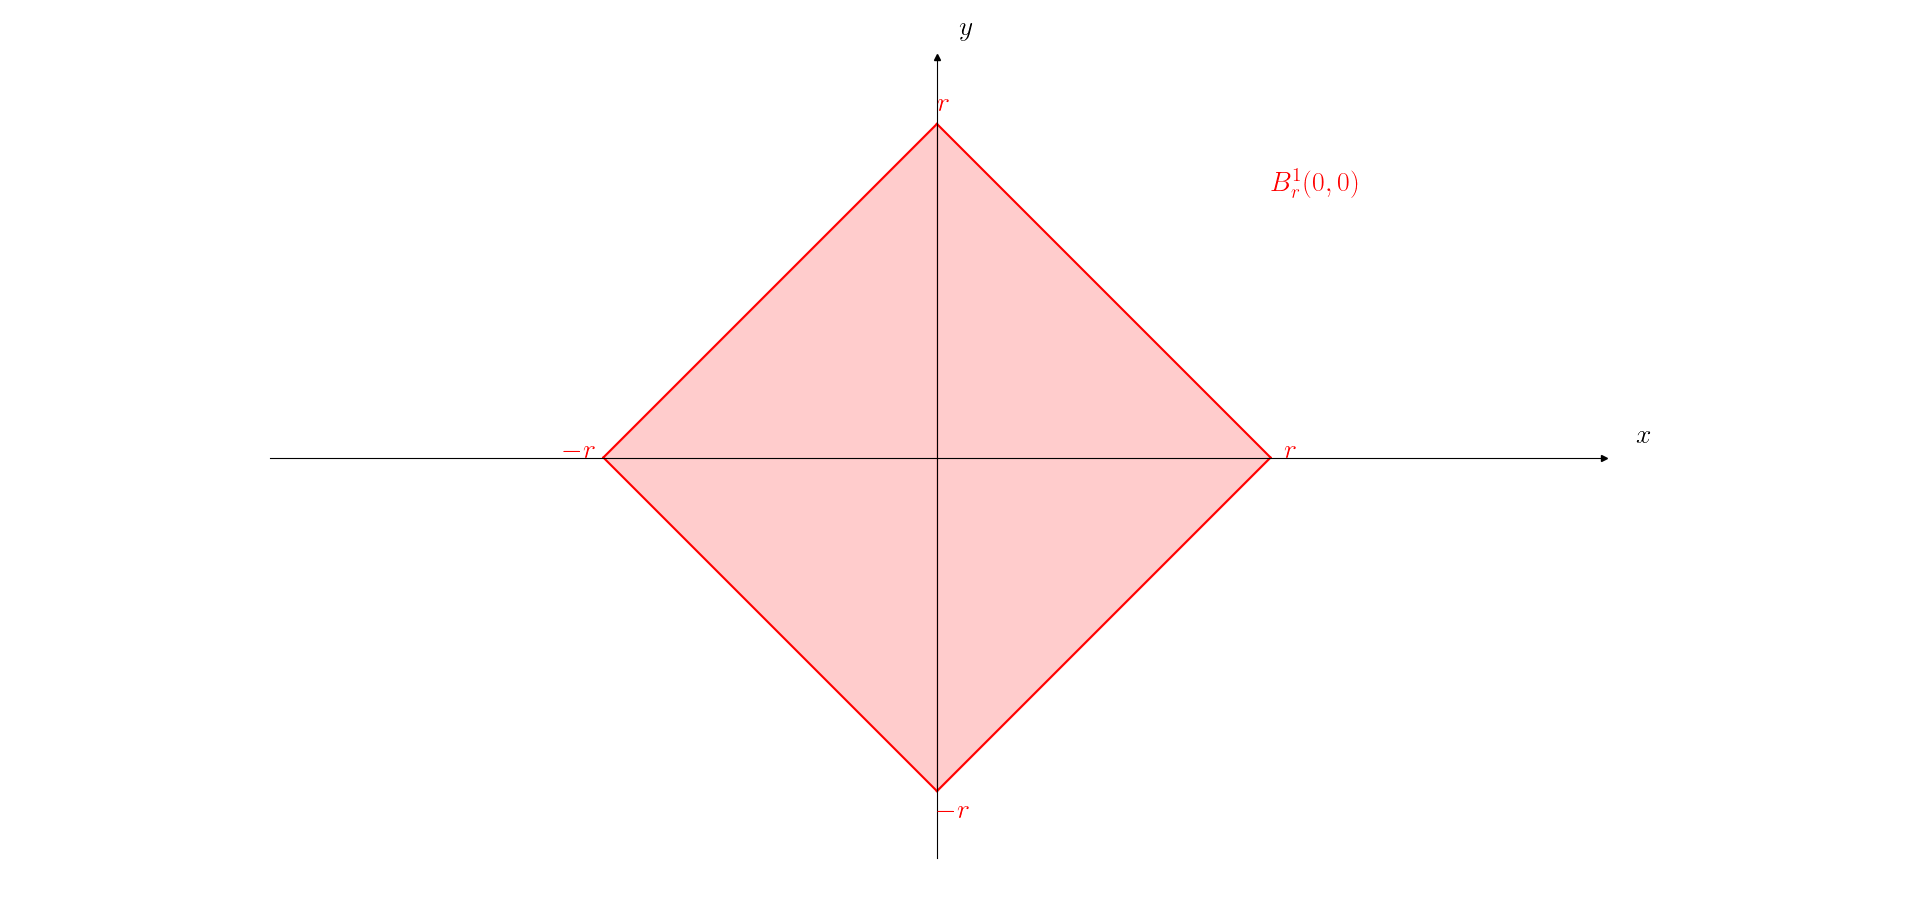
\includegraphics[width=0.75\linewidth]{spazi_metrici_e_normati/pag138rhombus}
		\label{fig:pag138rhombus}
	\end{center}

	\begin{gather*}
		(C^\circ([0,1]), \parallel \cdot \parallel_\infty) \qquad
		d(f,g) = \parallel f-g \parallel_\infty
		\\
		f \in C^0 (), \qquad r>0
		\\
		B_r^\infty(f) = \{ g \in C^0 ([0,1]) \big| \parallel f-g \parallel_\infty < r \} = \{ g \in C^0 ([0,1]) \big| \undercomment{\sup_{x \in [0,1]} |f(x) - g(x)|} {f(x) - r < g(x) < f(x) + r} {} < r \} 
	\end{gather*}		
	\begin{center}
		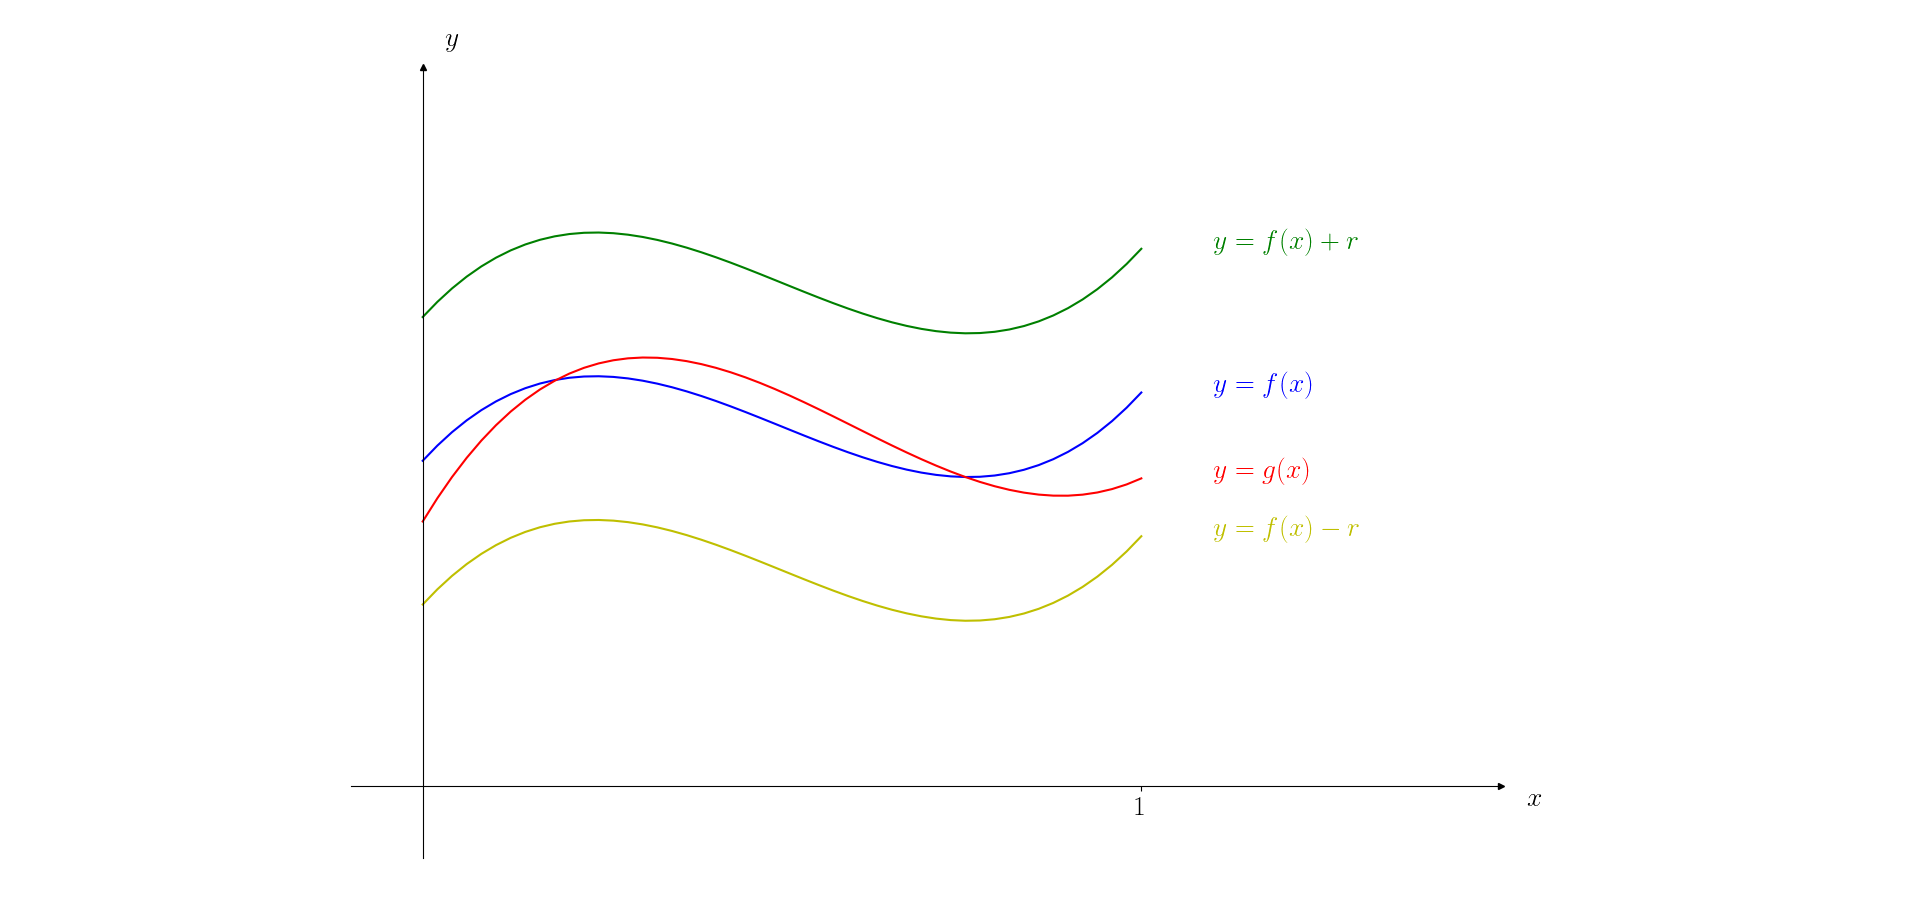
\includegraphics[width=0.75\linewidth]{spazi_metrici_e_normati/pag138curve}
		\label{fig:pag138curve}
	\end{center}
	
	$$f(x)=0 \qquad \forall \ x \in [0,1]$$
	\begin{center}
		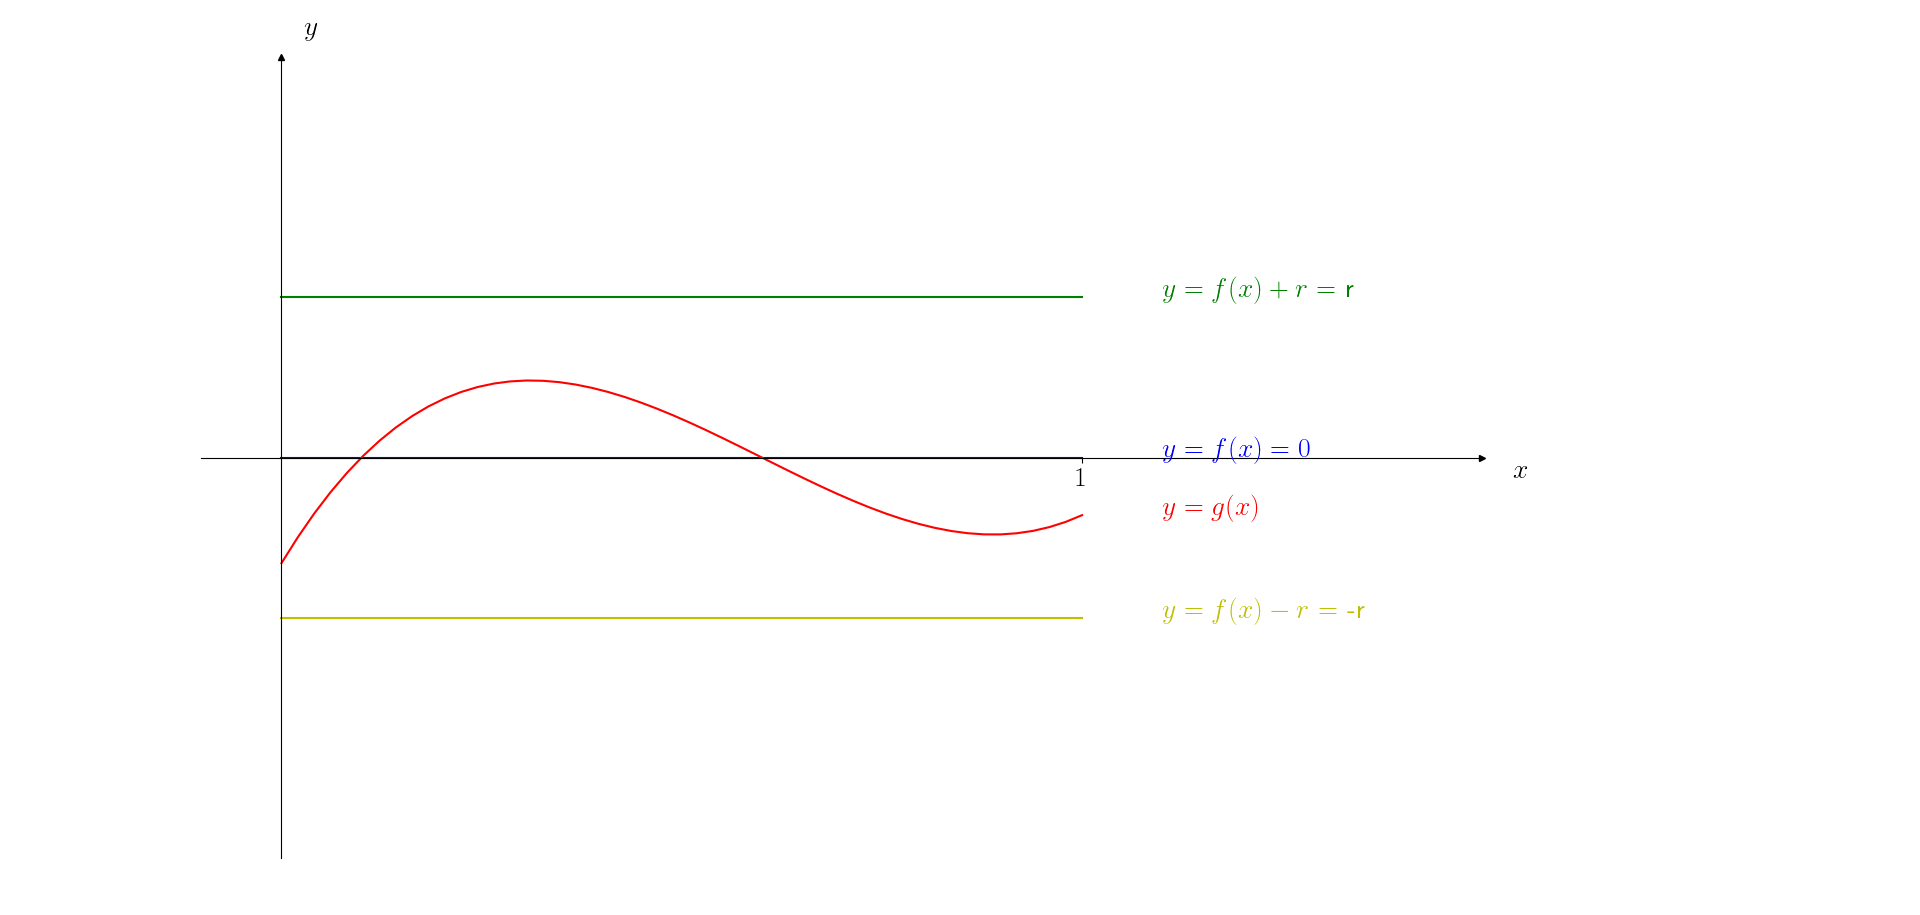
\includegraphics[width=0.65\linewidth]{spazi_metrici_e_normati/pag139curve}
		\label{fig:pag139curve}
	\end{center}
	
	\begin{gather*}
		C^0 ([0,1]), \parallel \cdot \parallel_1
		\\
		\parallel f \parallel_1 = \int_{0}^{1} |f(x)| \ \mathrm{d}x 
		\\
		B_r^1 = \{ g \in C^0 ([0,1]) \big| \parallel f-g \parallel_1 < r \} = \{g \in C^0 ([0,1]) \bigg| \int_{0}^{1} |f(x) - g(x)| \ \mathrm{d}x < r \}
		\\
		f(x) = 0 \qquad \forall \ x \in [0,1]
		\\
		B_r^1(0) = \{ g \in C^0 ([0,1]) \bigg| \int_{0}^{1} |g(x)| \ \mathrm{d}x < r \}
	\end{gather*}
	\begin{center}
		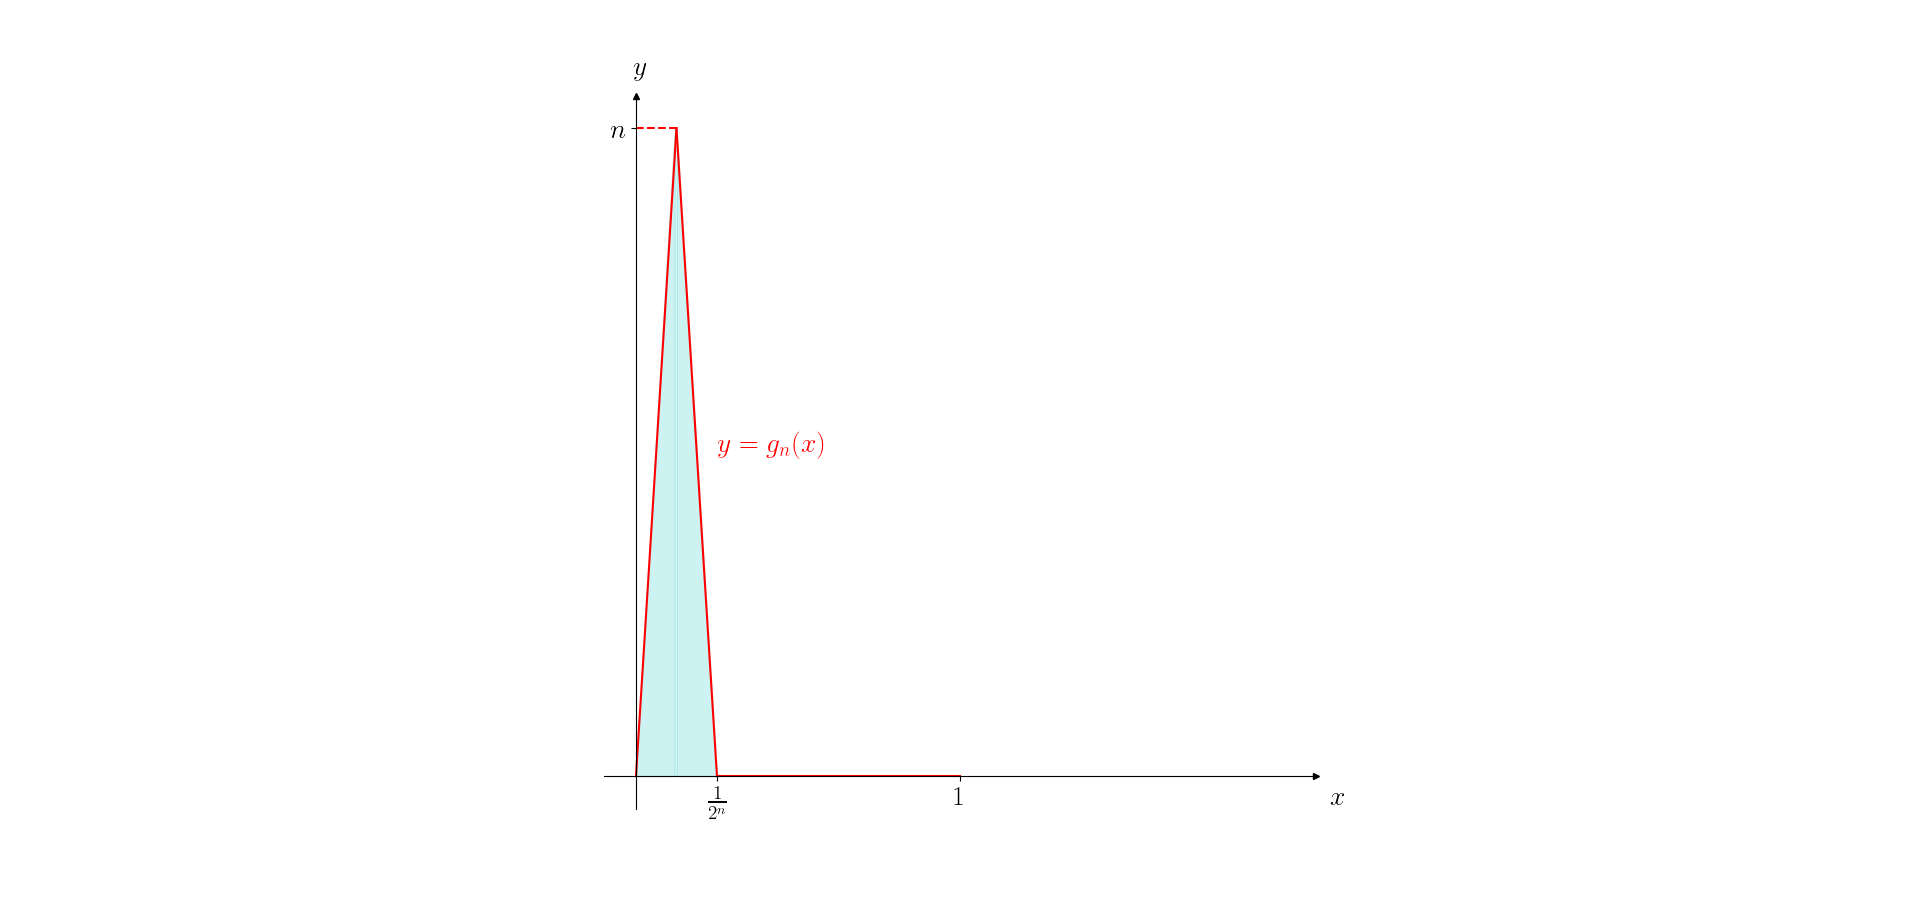
\includegraphics[width=0.85\linewidth]{spazi_metrici_e_normati/pag139triangolo}
	\end{center}

	$\int_{0}^{1} |g_n(x)| \ \mathrm{d}x =$ area del triangolo $ = \frac{1}{2} \frac{1}{2^n} n = \lowercomment{\frac{n}{2^{n+1}}} {\myarrow[270]} {0 \text{ per } n \rightarrow + \infty}$

	Fissato $r > 0$, trovo $n$ tale che $\int_{0}^{1} |g_n(x)| \ \mathrm{d}x < r$	
\end{exbar}


\begin{definition}
	$x \in X$. Un \textbf{intorno di $x$} è un qualsiasi sottoinsieme $A \subseteq X$ che contiene una palla aperta centrata in $x$, cioè per cui $\exists \ r > 0 \big| B_r(x) \subseteq A$
\end{definition}


\begin{definition}
	$A \subseteq X$ si dice \textbf{aperto} se è intorno di ogni suo punto, cioè se $\forall \ x \in A \quad \exists r > 0 \ \big| \ B_r(x) \subseteq A$.
	
	$A$ si dice \textbf{chiuso} se $A^c = X \backslash A$ è aperto.
\end{definition}


\begin{exbar}
\begin{example}
	$(x,d)$ spazio metrico, $x \in X, r>0$, $B_r(x)$ è un aperto.
	
	Devo far vedere che $\forall \ y \in B_r(x) \ \exists \ \overline{r} > 0 \ \big| \; B_{\overline{r}}(y) \subseteq B_r(x)$
	
	$\overline{r} = r - d(x,y) > 0$ perché $d(x,y) < r$ e dimostriamo che, se $z \in B_{\overline{r}} (y)$, allora $z\in B_r(x)$, cioè, se $d(y,z)< \overline{r}$, allora $d(x,z)<r$
	
	$d(x,z) \distr  d(x,y) + d(y,z) < d(x,y) + \overline{r} = d(x,y) + (r-d(x,y)) = r$	
	\begin{center}
		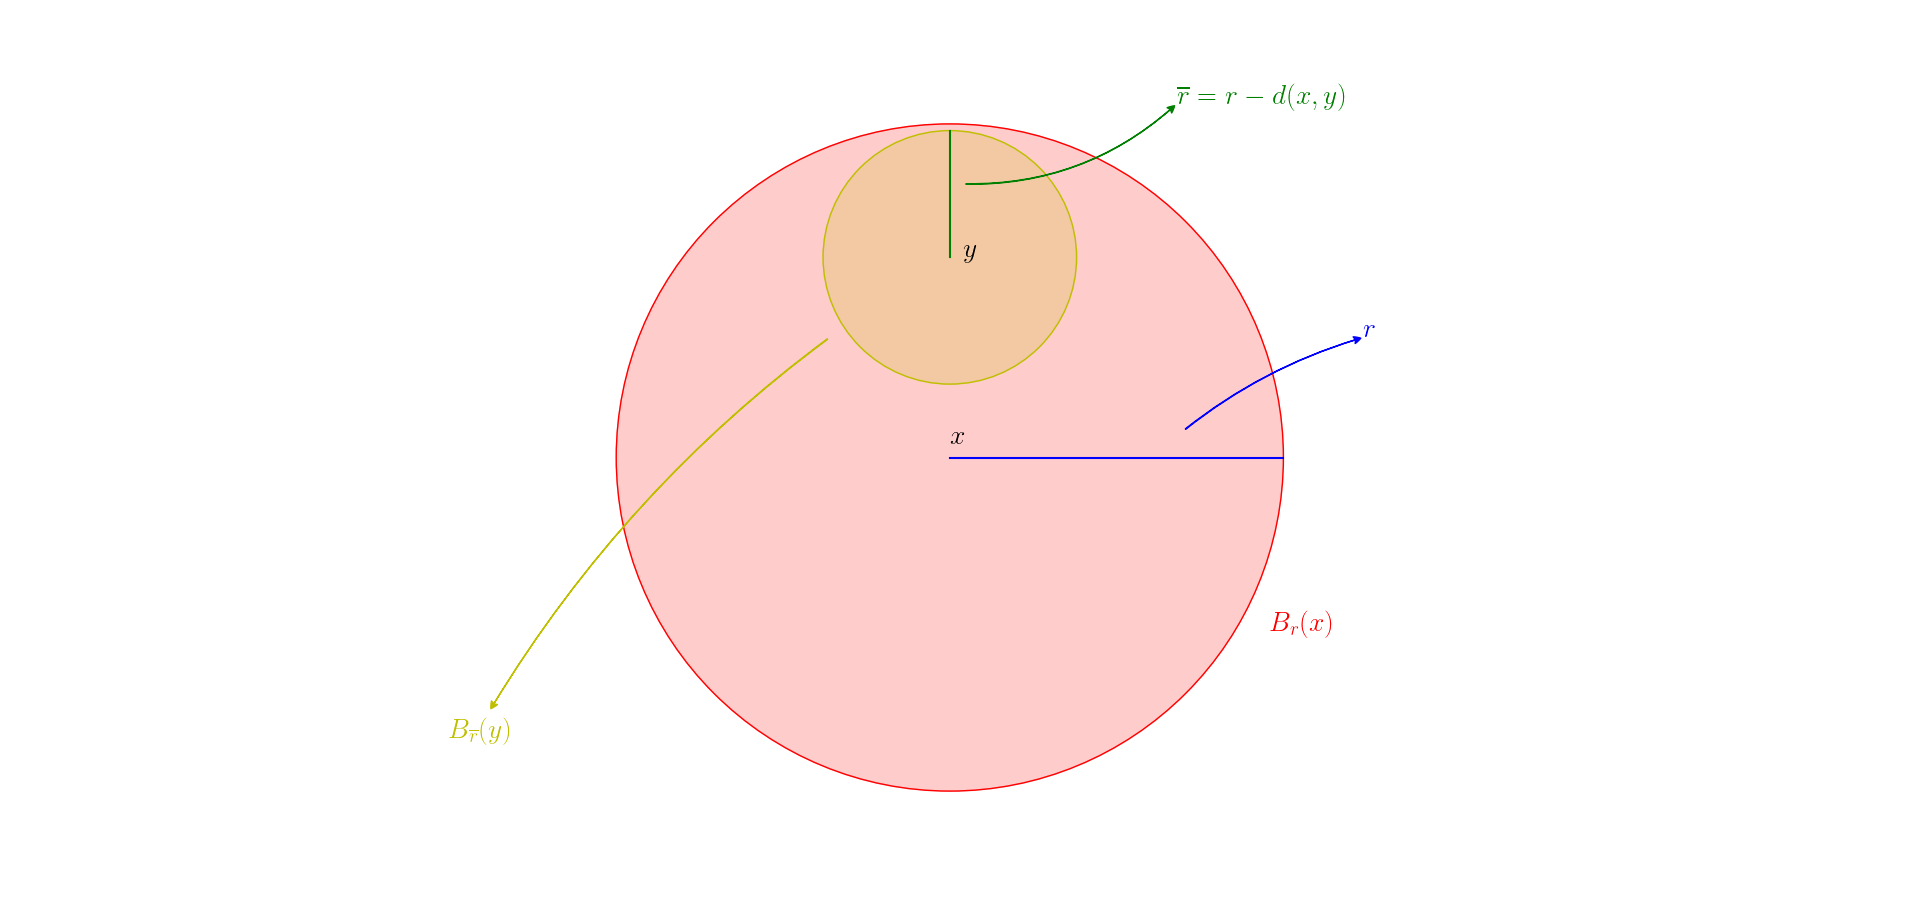
\includegraphics[width=0.75\linewidth]{spazi_metrici_e_normati/pag141}
		\label{fig:pag141}
	\end{center}
\end{example}
\end{exbar}


\begin{exbar}
	$(\mathbb{R}^2, \parallel \cdot \parallel_\infty)$
	\begin{center}
		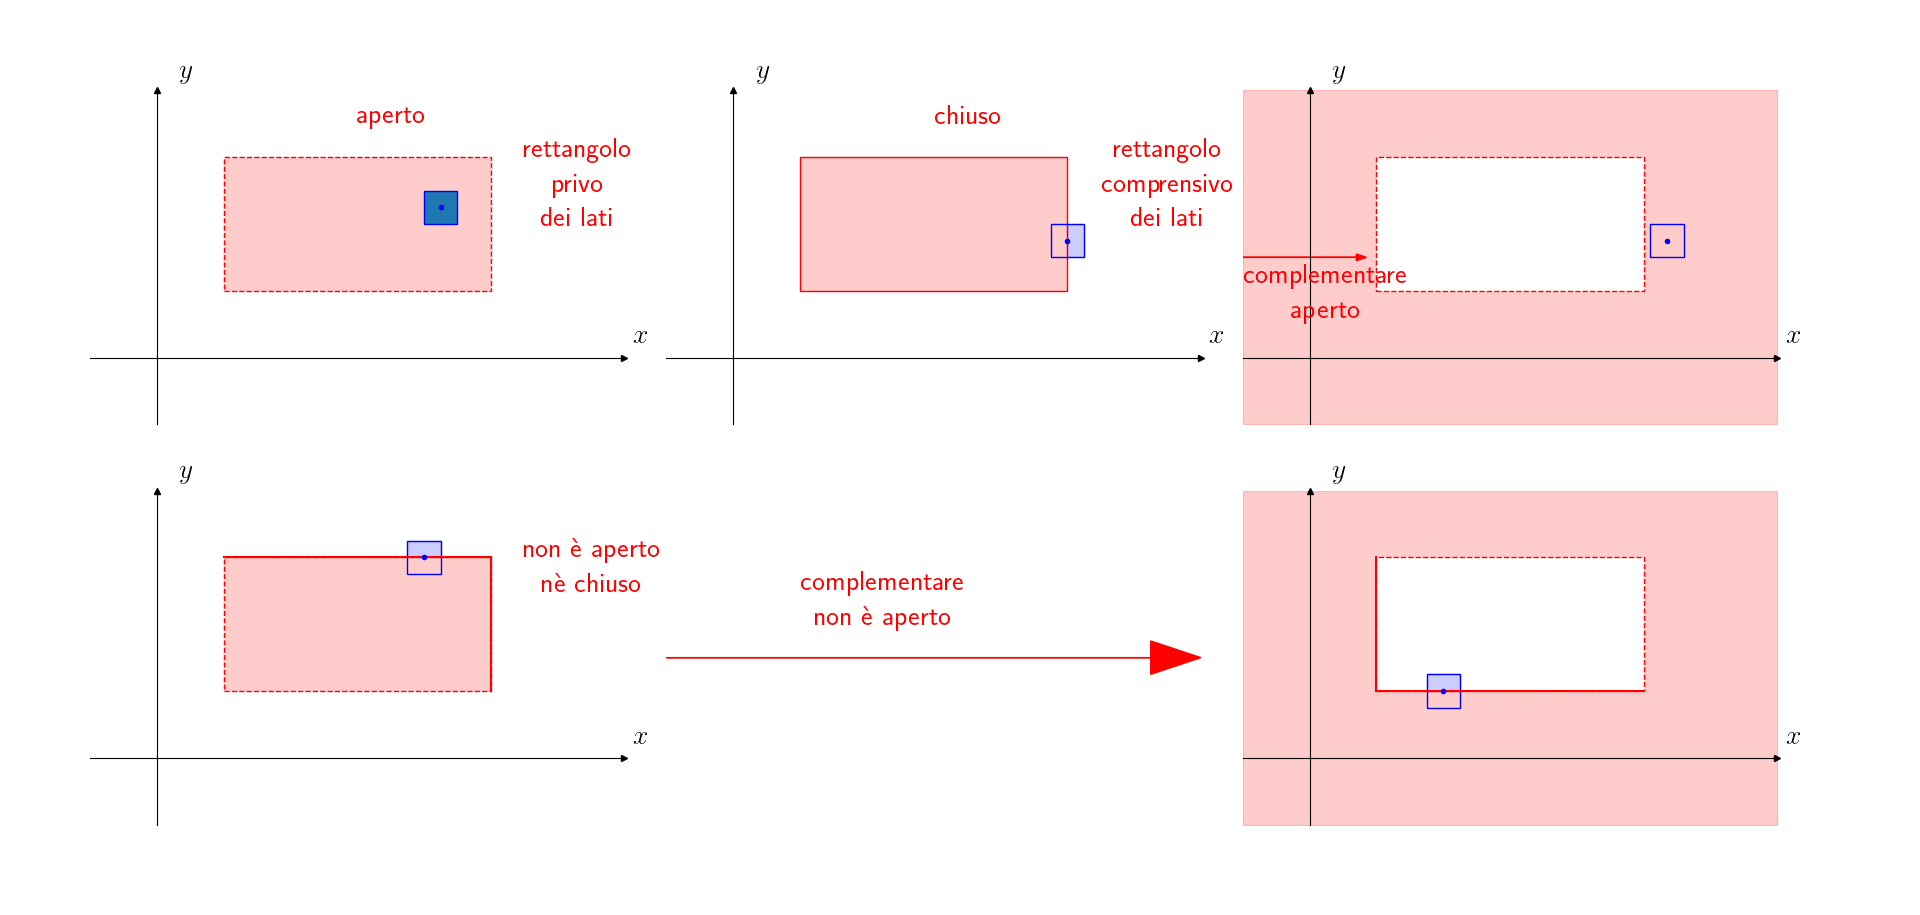
\includegraphics[width=\linewidth]{spazi_metrici_e_normati/pag141-142}
		\label{fig:pag141-142}
	\end{center}
\end{exbar}


\textbf{Osservazione:} 
	$(X,d)$ spazio metrico, $X$ è aperto banalmente (se $x \in X, B_r(x) \subseteq X \ \forall \ r > 0$) e quindi $\emptyset = X^c = X \backslash X$ è chiuso. 
	
	D'altra parte $\emptyset $ è aperto perché l'implicazione $x \in \emptyset \Rightarrow  \ \exists \ r > 0 \ \big| \ B_r(x) \subseteq \emptyset$ è vera perché $x \in \emptyset$  è falsa $\Rightarrow \emptyset^c = X \backslash \emptyset = X$ è chiuso. 
	
	\begin{attbar}
		$\emptyset, X$ sono sia aperti che chiusi.
	\end{attbar}


\begin{theorem}
	
	$(X,d)$ spazio metrico
	\begin{enumerate}
		\item $A_1, A_2 \subseteq X$ aperti $\Rightarrow A_1 \cap A_2$ è un aperto.
		 
		\item $\{A_i\}_{i \in I}$ è una famiglia di aperti, allora $\bigcup_{i \in I} A_i$ è un aperto.
		
		\item Se $C_1, C_2 \subseteq X$ sono chiusi, allora $C_1 \cup C_2$ è chiuso.
		
		\item $\{C_i\}_{i\in I}$ è famiglia di chiusi, allora $\bigcap_{i \in I} C_i$ è un chiuso.
	\end{enumerate}
\end{theorem}


\textbf{Osservazione:} 
In generale se $\{ A_i \}_{i \in I}$ è una famiglia infinita di aperti, allora $\bigcap_{i \in I} A_i$ non è un aperto e, se $\{ C_i \}_{i \in I}$ è una famiglia infinita di chiusi, allora $\bigcup_{i \in I} C_i$ non è chiuso. Facciamo un esempio.

$A_k= \ \bigg]-\frac{1}{k}, \frac{1}{k} \bigg[ \qquad k \geq 1, k \in \mathbb{N}$ sono tutti aperti di $\mathbb{R}$, allora $\bigcap_{k=1}^\infty A_k = \bigcap_{k=1}^\infty \ \bigg] -\frac{1}{k}, \frac{1}{k} \bigg[ \ = \{ 0 \}$, che è un chiuso.

$C_k = \left[ \frac{1}{k}, 1-\frac{1}{k} \right], \qquad k \geq 2, k \in \mathbb{N}$ sono tutti chiusi 

\bigg( $C_k^c = \ \bigg] -\infty, \frac{1}{k} \bigg[ \ \cup \ \bigg] 1-\frac{1}{k}, +\infty \bigg[$, unione di due intervalli aperti \bigg)

$\bigcup_{k=2}^\infty C_k = \bigcup_{k=2}^\infty \left[ \frac{1}{k}, 1-\frac{1}{k} \right] = \ ]0,1[$

Infatti, se $x \in \bigcup_{k=1}^\infty \left[ \frac{1}{k}, 1-\frac{1}{k} \right]$, allora $\exists \ \overline{k} \geq 2 \ \big| \ \left[\frac{1}{k}, 1-\frac{1}{k}\right]$, cioè $0 < \frac{1}{k} \leq x \leq 1- \frac{1}{k} < 1$

$\Rightarrow 0 < x < 1 \Rightarrow x \in \ ]0,1[.$

D'altra parte, se $x \in \ ]0,1[$, esistono $k_1$ e $k_2 \ \big| \ \frac{1}{k_1} < x<1 - \frac{1}{k_2}$

$k=\max\{k_1, k_2\}$ 

\begin{gather*}
	\frac{1}{k} \leq \frac{1}{k_1} < x < 1 - \frac{1}{k_2} \leq 1 - \frac{1}{k}
	\\
	\Rightarrow x \in C_k = \left[ \frac{1}{k}, 1 - \frac{1}{k} \right]
	\\
	\Rightarrow x \in \bigcup_{k=2}^{\infty} C_k
\end{gather*}


\begin{definition}
	
	$(X,d)$ spazio metrico, $A \subseteq X, \ x \in A$. $x$ si dice \textbf{punto interno di A} se $\exists \ r > 0 \ \big| \ B_r(x) \subseteq A$. L'interno di $A$ è l'insieme dei punti interni di $A$ ed è indicato con \AA
\end{definition}


\begin{proposition}
	\label{pr: grande aperto}
	\AA \ è un insieme aperto ed è il più grande aperto, nel senso dell'inclusione, contenuto in $A$, cioè se $B \subseteq A$ è aperto, allora $B \subseteq \AA$
\end{proposition}

\begin{dembar}
	\textbf{Dimostrazione} della \textbf{Proposizione \ref{pr: grande aperto}} (Esercizio per casa)
\end{dembar}


\begin{exbar}
	\begin{gather*}
		A = \ ]0,1], \qquad \AA = \ ]0,1[
		\\
		A = \ ]0,1] \cup \{ 2 \}, \qquad \AA = \ ]0,1[
		\\
		A = \ ]0,1] \cup \left\{2 + \frac{1}{n} \ \bigg| \ n \geq 1, n \in \mathbb{N} \right\}, \qquad \AA = \ ]0,1[
	\end{gather*}
\end{exbar}


\begin{definition}
	$A \subseteq X, x \in X$ si dice \textbf{punto di chiusura} per $A$ se $B_r(x) \cap A \neq \emptyset \ \forall \ r > 0$, cioè ogni palla di centro $x$ interseca $A$. 
	
	La chiusura di $A$ è l'insieme di tutti i punti di chiusura di $A$ ed è denotata con $\overline{A}$.
\end{definition}


\begin{proposition}
	\label{pr: grande chiuso}
	$\overline{A} $ è un insieme chiuso ed è il più piccolo chiuso, nel senso dell'inclusione, contenente $A$, cioè, se $C \geq A$ è chiuso, allora $\overline{A} \subseteq C$
\end{proposition}


\begin{dembar}
	\textbf{Dimostrazione} della \textbf{Proposizione \ref{pr: grande chiuso}} (Esercizio per casa)
\end{dembar}


\begin{exbar}
	\begin{gather*}
		A = \ ]0,1], \qquad \lowercomment{\overline{A} = [0,1]} {0 \notin A, \text{ mentre se } x \in \AA \Rightarrow x \in A} {x \in A \Rightarrow x \in \overline{A} \text{ perché } x \in B_r(x) \cap A \ \forall r > 0}
		\\
		A = \ ]0,1] \cup \{ 2 \}, \qquad \overline{A} = [0,1] \cup \{ 2 \}
		\\
		A = \ ]0,1] \cup \left\{ 2 + \frac{1}{n} \ \bigg| \ n \geq 1, n \in \mathbb{N} \right\}, \qquad \overline{A} = [0,1] \cup \left\{2 + \frac{1}{n} \ \bigg| \ n \geq 1, n \in \mathbb{N} \right\} \cup \{ 2 \}	\end{gather*}
\end{exbar}


\textbf{Osservazione:}
\begin{gather*}
	\AA \subseteq A \subseteq \overline{A}
	\\	
	A \text{ è aperto } \iff A = \AA
	\\
	A \text{ è chiuso } \iff A = \overline{A}
\end{gather*}

$(\Leftarrow) A=\overline{A}$, $\overline{A}$ è un chiuso $\Rightarrow A$ è chiuso

$(\Rightarrow)$ Sia $A$ chiuso e dimostriamo che $A = \overline{A}$. Noi sappiamo che $A \subseteq \overline{A}$.

Se per assurdo $A \nsubseteq \overline{A}, \; \exists \ x \in \overline{A} \ \big| \ x \notin A$, cioè $x \in \overline{A}$ e $x \in A^c$. Ma $ A^c $ è aperto, perché $ A $ è chiuso, e quindi $ \exists r > 0 \ \big| \ B_r (x) \subseteq A^c$

$\Rightarrow B_r (x) \cap A = \emptyset$, assurdo perché $x \in \overline{A}$.


\begin{definition}
	$A \subseteq X, x \in X$ si dice \textbf{punto di frontiera} per $A$ se $\forall \ r > 0 \quad B_r(x) \cap A \neq \emptyset$ e $B_r(x) \cap A^c \neq \emptyset$, cioè se ogni palla di centro $x$ interseca sia $A$ che il suo complementare.
	
	L'insieme dei punti di frontiera di $A$ si dice frontiera di $A$ e si indica con $\partial A$. 
\end{definition}


\begin{exbar}
	\begin{gather*}
		A = ]0,1], \qquad \partial A = \{0,1\} 
		\\
		A = \ ]0,1] \cup \{ 2 \}, \qquad \partial A = \{ 0, 1, 2 \}
		\\
		A = \ ]0,1] \cup \left\{ 2 + \frac{1}{n} \ \bigg| \ n \geq 1, n \in \mathbb{N} \right\}, \qquad \partial A = \{0,1\} \cup \left\{2 + \frac{1}{n} \ \bigg| \ n \geq 1, n \in \mathbb{N} \right\} \cup \{ 2 \}
	\end{gather*}
$(\mathbb{R}^2, \parallel \cdot \parallel_\infty)$
g
\begin{center}
	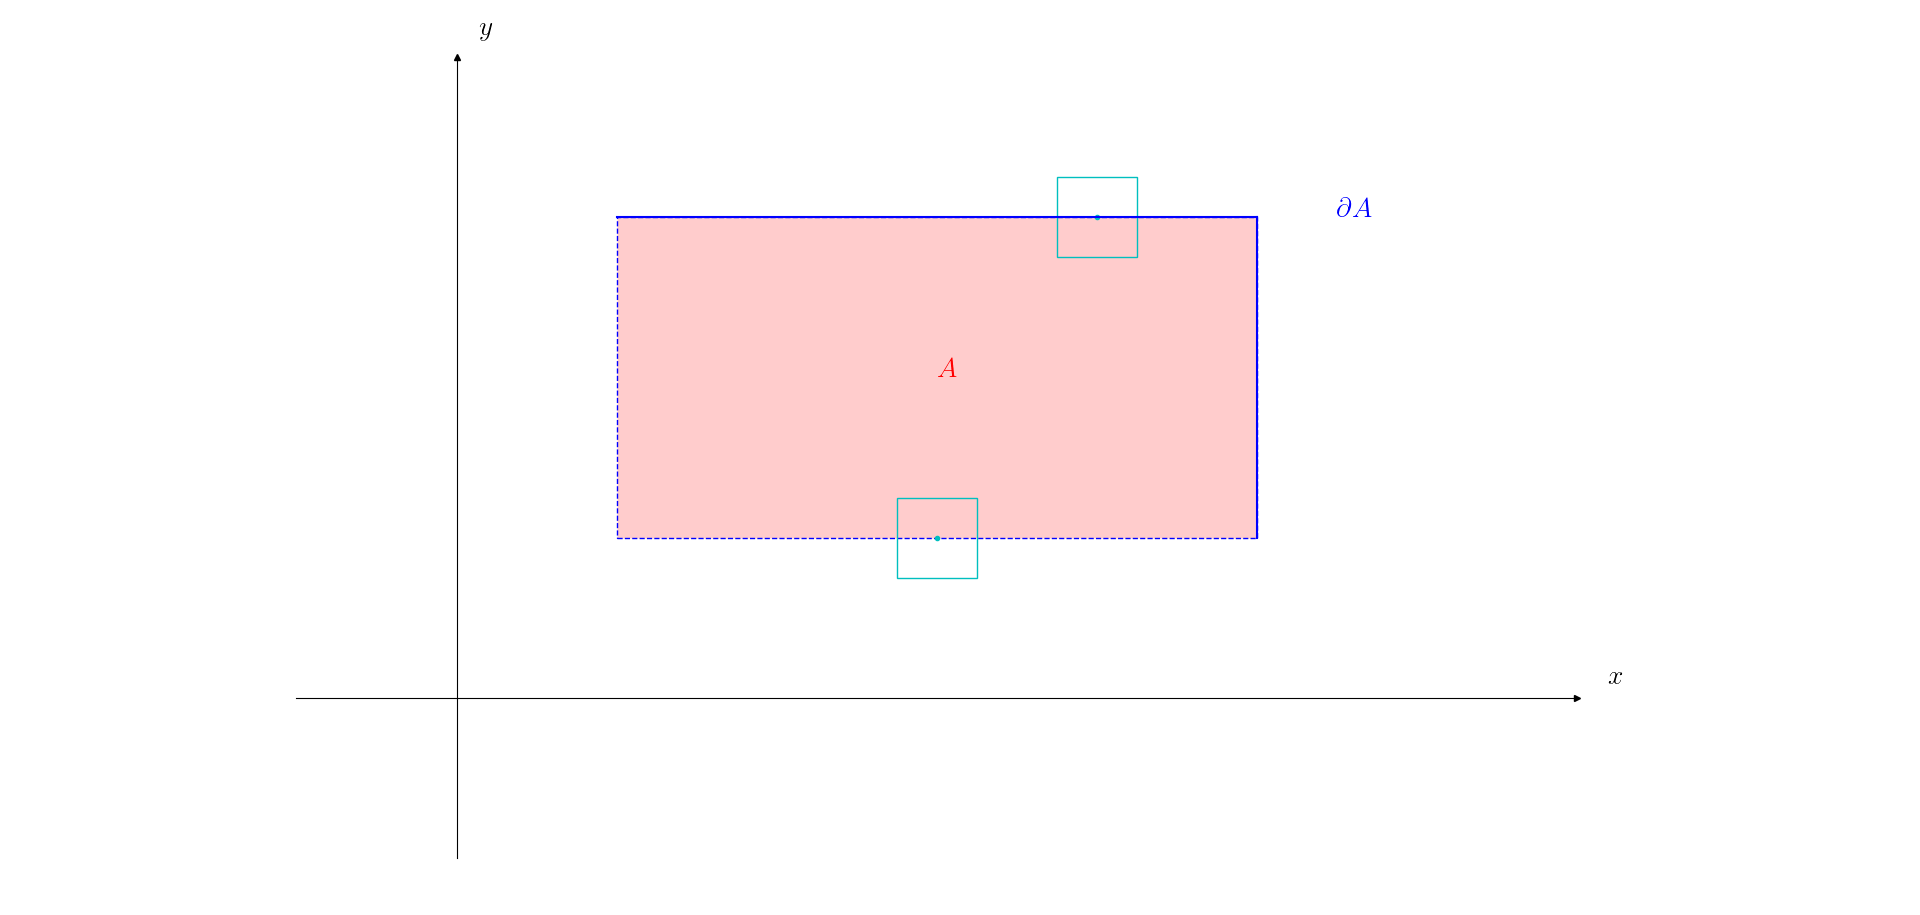
\includegraphics[width=0.65\linewidth]{spazi_metrici_e_normati/pag148}
	\label{fig:pag148}
\end{center}
\end{exbar}





\begin{comment}	


	
	
	
	
\end{comment}